\section{Деградация РТГС на основе $Al_{x}Ga_{1-x}As$}

Ранее было выявлено, что доминирующим фактором деградации при производстве РТГС является высокотемпературный отжиг, а при эксплуатации доминирует проникновение легирующей примеси в активную область через $10$ лет для исследуемой модели.

Таким образом в первые 10 лет ВАХ РТГС определяет деградация при обжиге, после этого срока проникновение легирующей примеси. На основании этих данных была написана программа (лист.\ref{lst:Degr}) учитывающая этих два параметра при моделирование деградации.

Исследуемая модель:
\begin{itemize}
	\item Спейсер: $a = 10$ монослоев;
	\item Барьер: $b = 6$ монослоев;
	\item Яма: $c = 6$ монослоев;
	\item Приконтактная область: $r = 20$ монослоев;
	\item Технологические фактор. Отжиг ГС ($t\approx30$ секунд, $T\approx800^{\circ}$C);
	\item Эксплуатационный фактор ($t\approx 13$ лет, $T\approx100^{\circ}$C);
	\item $N_{D}^{r} = 2*10^{23}$м$^{-3}$;
	\item $N_{D}^{r+} = 2.5*10^{24}$м$^{-3}$.
\end{itemize} 

\begin{figure}[h!]
	\centering
	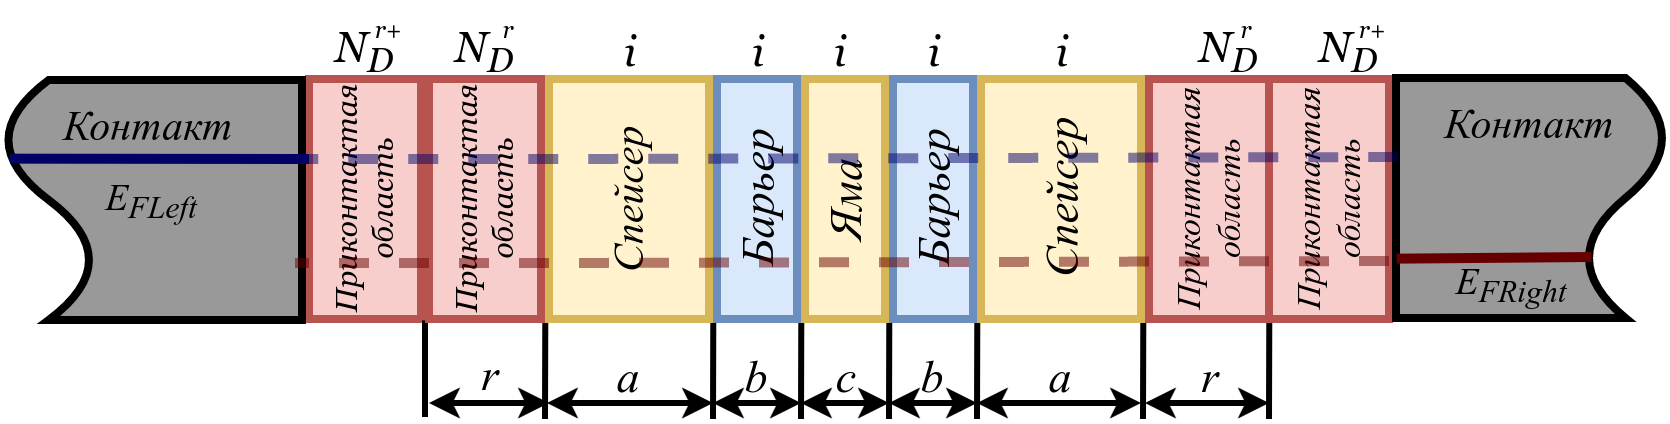
\includegraphics[width=.95\linewidth]{RTHSResearch}
	\caption{Модель исследуемой РТГС} 
	\label{fig:RTHSResearch}
\end{figure}

Результаты моделирования представлены на рис. \ref{fig:DegrC} и
рис. \ref{fig:DegrJ} получены с помощью лист.\ref{lst:Degr}.
\begin{figure}[h!]
	\centering
	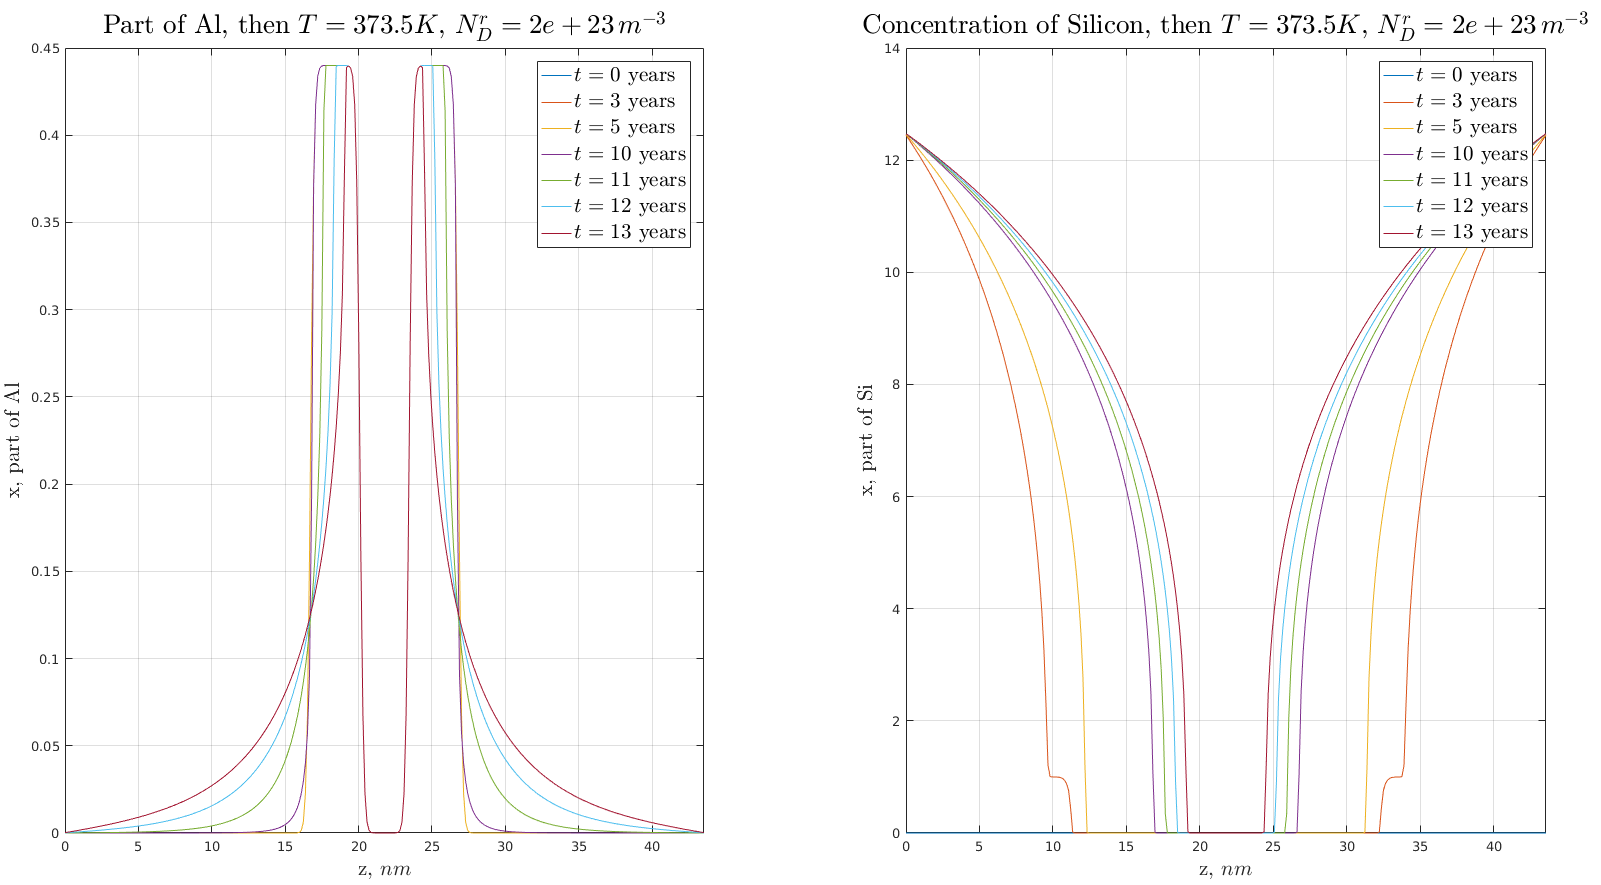
\includegraphics[width=.95\linewidth]{DegrC}
	\caption{Деградация профиля дна ЗП РТГС на $Al_{x}Ga_{1-x}As$}
	\label{fig:DegrC}
\end{figure}

\begin{figure}[h!]
	\centering
	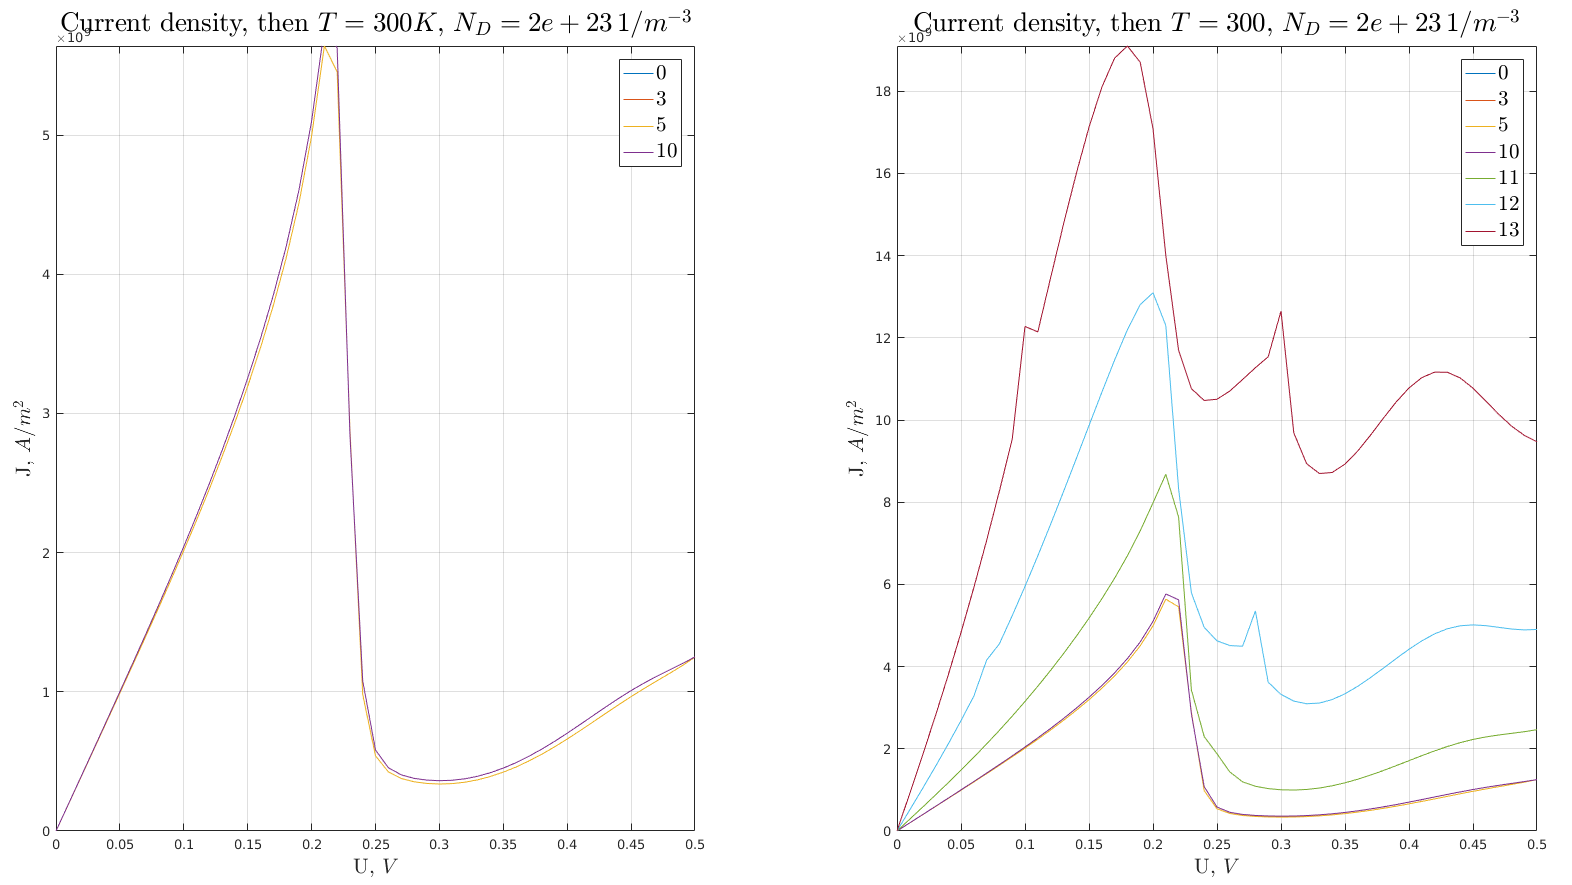
\includegraphics[width=.9\linewidth]{DegrJ}
	\caption{Деградация профиля дна ЗП РТГС на $Al_{x}Ga_{1-x}As$}
	\label{fig:DegrJ}
\end{figure}

\subsection{Вывод}
Получена алгоритм прогнозирования деградации РТГС на основе $GaAs$, в котором учтены доминирующие факторы, влияющие на ВАХ прибора на основе данной ГС. Основные факторы влияющие на деградацию:
\begin{itemize}
	\item Отжиг ГС при высокой температуре;
	\item Диффузия легирующей примеси в активную область.
\end{itemize}